% Bader Zaidan 2017, Aachen, Germany.
% This document is in the Creative Commons Attribution-NoDerivatives 4.0 International.
% You may share it and use it for commercial purposes as well, but do not share modifications of this work.

\title{%
	Firmware Password Extraction of Consumer Hewlett-Packard Laptops
	\\ \large HP PSR-2017-0169 \\ CVE-2017-2751
}
\author{Bader Zaidan \\ \\ \href{mailto:bader@zaidan.tech}{bader@zaidan.tech}} 

\date{November 1, 2017}
\documentclass[a4paper,12pt]{article}

\usepackage{courier}
\usepackage{hyperref}
\usepackage{graphicx}

\begin{document}
\maketitle
\begin{center}
\small{\href{https://support.hp.com/us-en/document/c05913581}{HP Security bulletin}}
\\\small{This work is licensed under a Creative Commons Attribution-NoDerivatives 4.0 International License.}
\\\small{Last update: 29.01.2018 - Added CVE and link to HP announcement}
\end{center}
\section{Introduction}
The BIOS password is one of the most basic methods of preventing manipulation of boot firmware settings and undesired manipulation of a device. Security measures in the boot firmware exist in virtually all modern devices and are considered to be an industry standard. Several exploits, bugs and other security issues already exist, but are ignored and are rarely taken advantage of due to their complexity. One that is simple to execute will provide an increased capability to even the smallest of assailants.


In this paper, we will cover a bug where an assailant can access the BIOS/UEFI password via the OS or any other method allowing him to read the CMOS memory. This issue was found in the European Coreboot Conference in Bochum, 2017.

\section{Reproduction}

Reproducing this issue requires nothing more than a tool capable of dumping the CMOS memory contents and possibly a program to read it in hexadecimal form. In this example, we tested the issue with \texttt{nvramtool} with option \texttt{-x} (allowing a hex dump, removing the need for a hexadecimal reader or editor) under Debian GNU/Linux 9.2. 

\begin{figure}[ht!]
	\centering
	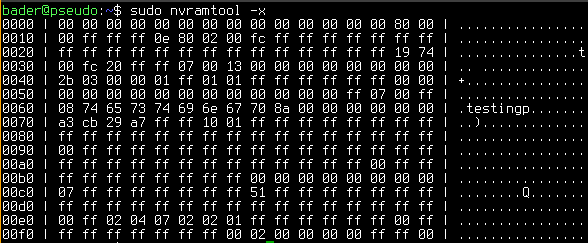
\includegraphics[width=120mm]{image.png}
	\caption{\texttt{nvramtool -x} output under GNU/Linux. \label{screenshot}}
\end{figure}

The password on this device was found to be between 0x0061 and 0x0068 inclusive of said dumps as shown in the figure. It remains unhashed, unsalted and unencrypted. For the sake of this demonstration, the password was set to "testingp". Note: The password was also limited to 8 characters and cannot be increased due to a hard limit.


\section{Affected Devices}
%%As of now, only the HP 14-r100nia (version K1P94EA\#BH5) with BIOS Insyde F.36 of release date 18.12.2014 was tested and leaked the set password. The HP 15-ay536ng (version Z9A06EA\#ABD) and an HP 625 (unknown firmware type) did not. More testing is needed to confirm if other makes or models with this BIOS release suffer from this bug. As of the day of writing of this paper, no security updates were released.
The list of affected devices is available on the HP Support Communications board found \href{https://support.hp.com/us-en/document/c05913581}{here.}

%%It is possible that there are more devices which suffer from this bug. More testing is needed to confirm.


\end{document}
